\documentclass[../main.tex]{subfiles}
\begin{document}
\subsection*{Orthodox Interpretation of Quantum Mechanics}
From Young's experiment, we saw bright bands (lots of light) and dark bands (no light). The patch is being hit by light waves from both slits, out of phase with each other, causing destructive interference. The explanation relies on the fact that light waves spread out through space, traveling through both slits at once. 

The one photon at a time double-slit experiment result however suggest that photon is a particle that able to interference with itself. The interference pattern has a clear mathematical implication: a wave is spreading out from the two slits and then interfering with itself. But,what is waving? The classical answer is that an electric field and a magnetic field are both oscillating, and a high amplitude of the wave corresponds to high strengths of these two fields. But that answer would never lead to an individual spot at one point on the back wall. In 1926, Max Born proposed that the wave represents probabilities. A photon is a particle that hits the back wall in a particular spot, but associated with that particle is a wave that determines the probabilities of measuring that photon at various positions. 

The orthodox interpretation (Copenhagen interpretation) says that the particle exists as a wave, spread out throughout space, until the moment you measure it. At that moment the wave “collapses” into a state of being in one particular place. 

\subsection*{Photoelectric Effect}
Consider two metal plates in a vacuum. Plate B is large and is bent around Plate A. Voltage source sets up a potential difference such that $V_A > V_B$. Due to potential difference, electrons on Plate A are certainly not going to jump to Plate B. Now suppose that we shine a beam of ultraviolet light onto Plate A. Such a beam can transfer energy to electrons in the metal, and an electron that absorbs enough energy will escape from the metal entirely. 

\begin{figure*}[b]
    \centering
    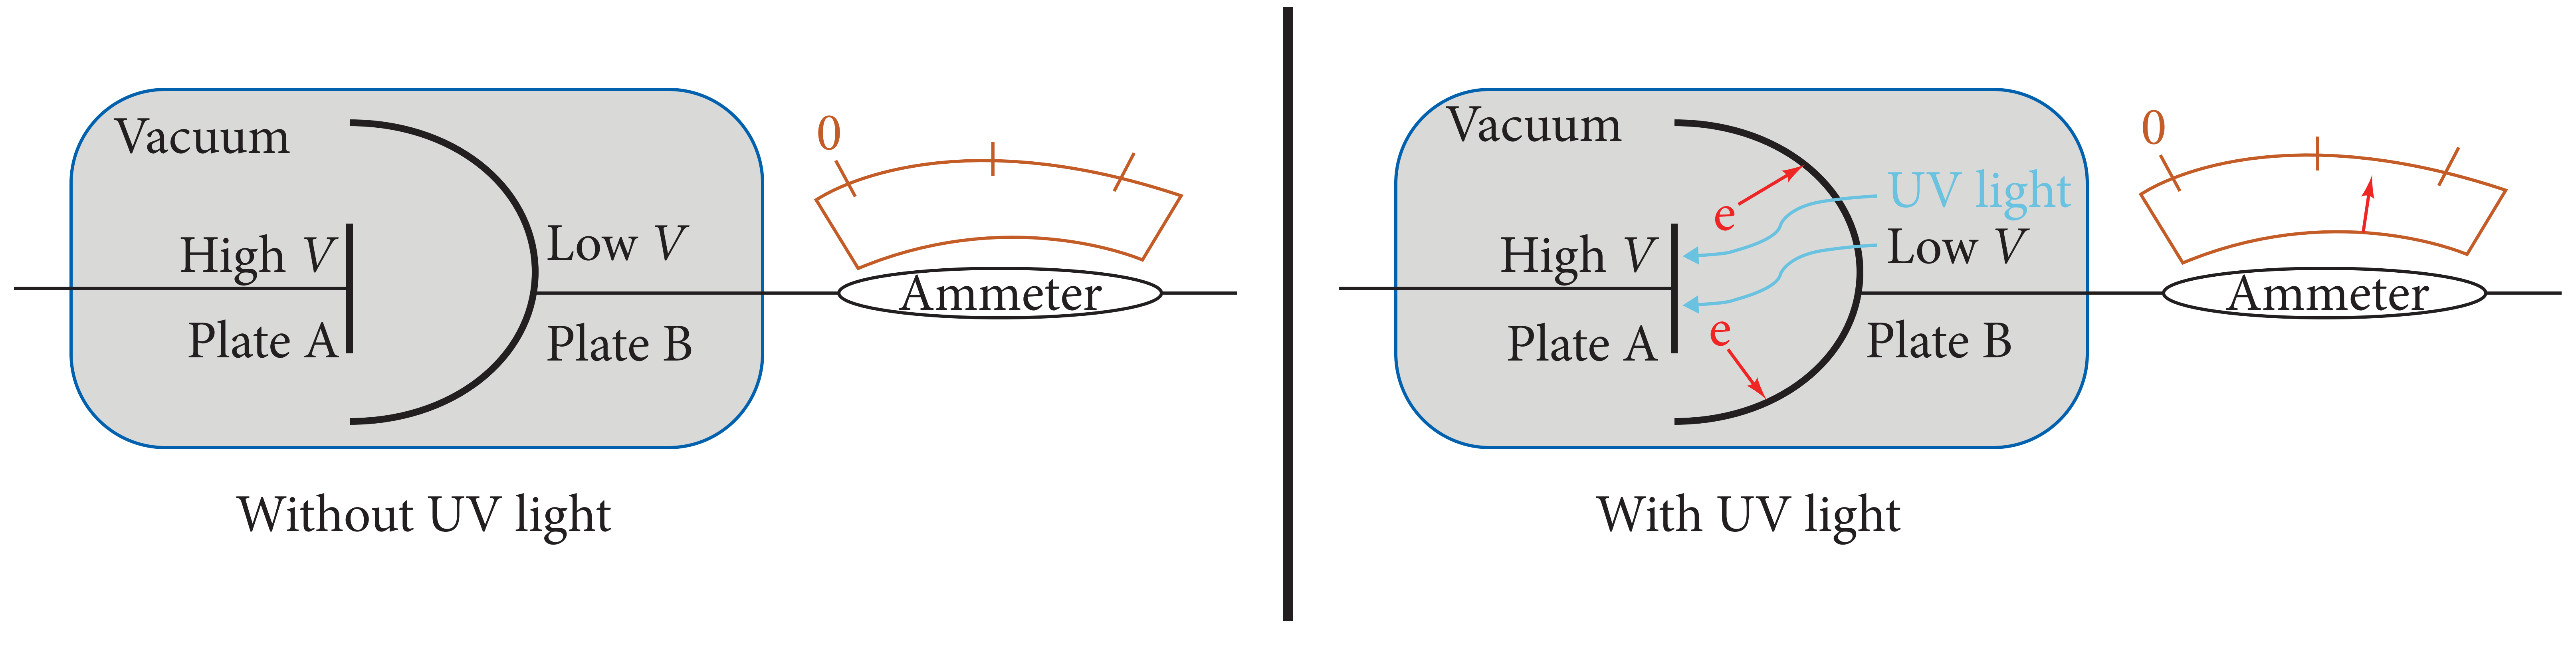
\includegraphics[width=\textwidth]{../Rss/QM/Chapter/PhotoElec.png}
    \caption*{Figure: Photoelectric experiment}
\end{figure*}

The required energy $w$ for an electron to initially escape Plate A depends on how tightly bound the electron is to its atom, and on how close it is to the surface. After escaping Plate A, the electron will need to fight the electric field; the required kinetic energy for a charge $e$ to cross a voltage gap $V$ is $eV$. Thus, total energy required for an electron to escape Plate A and reach Plate B is 
\begin{equation*}
    E_{A\rightarrow B}=w+eV
\end{equation*}
Only the ones with $K \geq Ve$ make it to Plate B; if the maximum kinetic energy of any escaped electron
is below $eV$ then the current stops completely. So by increasing the potential gap until we find the the potential difference that stops all current $V_0$, we can calculate the maximum kinetic energy with which any electron leaves Plate A
\begin{equation*}
    K_{\text{max}}=eV_0
\end{equation*}

We will show the result of the experiment, and the we will compare how classical electrodynamics versus quantum mechanics prediction; which, as you know, classical electrodynamics got some wrong.
\begin{enumerate}
    \item Intensity of the light proportional to the resulting current.
    \item $K_{\text{max}}$ is independent of the light intensity.
    \item $K_{\text{max}}$ is a function of frequency: electrons liberated by high-frequency light have more kinetic energy than electrons liberated by low-frequency light. Furthermore, there is a cutoff frequency; in which light below this frequency liberates no electrons.
    \item No time lag is observed, no matter how low the intensity of the radiation. 
\end{enumerate}

Classically, the energy of that wave is a function of its intensity, which is to say, of the amplitude. The amount electron liberated, thus current, therefore proportional to that wave energy, thus intensity. Classical electrodynamics, however, only able to correctly predict that first item. Wrong classical electrodynamics are as follow: $K_{max}$ increase at higher intensities; frequency of the light have no effect on $K_{max}$; and a dim light should take a while to impart enough energy to liberate an electron, so there should be a measurable time lag before any current is detected.

Quantum mechanics, however, able correctly predict and explain the experiment. For the first item, according to quantum mechanics, a higher intensity beam has more photons per second, so more electrons get knocked out. 

There is a minimum possible value of $w$, for the electrons nearest the surface and most lightly bound to their atoms. That value, $w_0$ , is called the work function of the material on Plate A. The electrons that are easiest to knock free require a total energy $w_0 + eV $ to reach Plate B. If $h\nu$ is lower than $w_0 + eV$ then no electrons cross the gap to Plate B. This explains the cutoff frequency that is seen in experiment but is impossible to explain classically. For the lack of time lag, quantum mechanics explains that some electrons get hit by a photon and instantly receive energy $h\nu$, while others aren't hit and receive zero energy; so as soon as photons strike Plate A, electrons are liberated.

\subsection*{Atomic Models}
\subsubsection*{Thomson's model.} In 1897, J. J. Thomson showed that atoms contain electrons, negatively charged particles much smaller and lighter than the atoms themselves. Since atoms are generally neutral, there had to be something to cancel that negative charge, and to account for most of the mass of the atoms. In 1904, Thomson proposed that the electrons in an atom were embedded in a uniform spherical distribution of positive charge; this description is called the plum pudding model of the atom because the electrons are distributed in the atom like raisins in a plum pudding.

\subsubsection*{Rutherford's model.} That model was conclusively disproven in 1911 when Ernest Rutherford fired high-energy alpha particles at a thin gold foil. Electrons are too light to significantly deflect alpha particles, so any observed deflection resulted from interactions with the positive charges in the atom. Rutherford observed some alpha particles recoiled at angles greater than 90 degrees, which would have been essentially impossible in Thomson's model. 

Rutherford concluded that instead of being embedded in a diffuse medium of positive charge, the electrons must orbit about a tiny ball of positive charge that he called the nucleus. An alpha particle that happens to strike almost exactly next to this small, dense nucleus experiences a large force and can recoil at a large angle.

But Rutherford's model faced two important problems. The first problem is stability. As you know, any orbiting object has a centripetal acceleration, thus lose energy and rapidly spiral into the nucleus. In fact, Maxwell's equations predict that a Rutherford-style hydrogen atom should last about $10^{-12} $ s. The second problem is atomic spectra. 

\subsubsection*{Bohr's Model.} Bohr's model described electrons orbiting a nucleus in circular orbits have quantized orbit and angular momentum equal to $nh/(2\pi)$. Electrons can jump discontinuously between allowed orbits. Such a jump will emit or absorb a photon whose energy is precisely the difference between the energies of those two orbits. Bohr's rule for quantized angular momentum quantized energy
\begin{equation*}
        E_n=-\frac{m_ee^4}{24(\pi\epsilon_0)^2\hbar^2}\frac{1}{n^2}=-\frac{1}{n^2}\text{Ry}
\end{equation*}
and quantized radius
\begin{equation*}
    r=\frac{\pi\epsilon_0\hbar^2}{m_ee^2}n^2=a_0n^2
\end{equation*}
with $\hbar=h/(2\pi)$. The energy unit “rydberg” (Ry) is roughly equal to 13.6 eV. The distance $a_0$ , called the “Bohr radius,” is about half an angstrom, or $5 \times 10^{-11}$ m. 

Negative sign in the energy formula caused by potential energy; which defined to be 0 when the electron is infinitely far away from the nucleus. Potential energy increases as you move away from the nucleus, which makes the potential energy negative at all finite distances. If the total energy $E = U + K$ is positive, the electron has enough energy to leave the atom completely, so for any orbiting electron $E$ will be negative. 

An electron dropping from level $n_2$ to level $n_1$ will emit photons with the frequencies predicted by the Rydberg formula. The Lyman series comes from electrons dropping from any of the higher levels into the ground state or $n=1$, the Balmer series comes from electrons dropping from higher levels into $n = 2$, the Pascen series comes from electrons dropping from higher levels into $n = 3$, the Brackett series comes from electrons dropping from higher levels into $n = 4$, the Pfund series comes from electrons dropping from higher levels into $n = 4$.

\subsection*{Atomic Spectra}
If you run a large electrical current through a tube filled with gas, the current gives energy to the atoms of that gas. The atoms then release that energy as electromagnetic radiation. If you put that radiation through a prism you find that it is not a uniform rainbow of colors. These colored lines are called “emission lines.” Each element emits a unique pattern known as its “emission spectrum.” The spatial frequencies of the emission lines of hydrogen are given by
\begin{equation*}
    f=\frac{1}{\lambda}=\text{R}_H\biggl(\frac{1}{n_1^2}-\frac{1}{n_2^2}\biggr)
\end{equation*}
Here $n_1$ can be any positive integer and $n_2$ can be any integer larger than $n_1$. Rydberg constant
for hydrogen R$_H$ = $1.10 \times 10 7$ m${^-1}$. The frequency (defined as one over the oscillation period $T$) of each line is $\nu = cf $.

\subsection*{Matter Waves}
Every particle has an associated “matter wave” with wavelength $ \lambda = h/p$. Sometimes people use “de Broglie relations” in the plural: the $ \lambda = h/p$, and also the equation $E = h\nu$ relating the total relativistic energy of a particle to its frequency. Note that the first involves a wavelength in space, the second a frequency in time.

\subsection*{Wavefunctions }
A particle moves through space as a wave that exists simultaneously throughout an extended region. Knowing the wavefunction does not in general allow you to predict the outcomes of measurements of the particle, instead it allows you to predict the probabilities of different measurements.

\subsubsection*{Probability.} For a discrete universe, is the probability of finding the particle at $x$ is
\begin{equation*}
    P(x)=|\psi(x)|^2
\end{equation*}
For a continuous distribution 
\begin{equation*}
    P(a\leq x \leq b)=\int_{a}^{b}|\psi|^2\;dx
\end{equation*}
the integral gives the probability of finding the particle between those two points. Notice that it's not probability, but a probability density.

\subsubsection*{Normalization.} A distribution in which all the probabilities add up to 1 is said to be “normalized.” 
\begin{equation*}
    \int_{-\infty}^{\infty}|\psi|^2\;dx=1
\end{equation*}
Any valid probability distribution must be normalized.

\subsubsection*{Expectation values.} In statistics the average you expect to get from measuring the same thing many times is called the “expectation value” of that measurement. For discrete universe
\begin{equation*}
    \langle x\rangle=\sum_{x}^{}xP(x)
\end{equation*}
for continuous universe
\begin{equation*}
    x=\int_{-\infty}^{\infty}x|\psi|^2\;dx
\end{equation*}
applies to any discrete normalized probability distribution $P(x)$

\subsection*{Schrödinger's Equations }
\subsubsection*{Energy Eigenstates.} If a particle's wavefunction $\psi$ is an “energy eigenstate” (also called “energy eigenfunction”), then the particle has a definite energy. That is, there is a 100 $\%$ chance of finding that particular energy, and zero chance of finding any other. That particular energy is called the “eigenvalue” of that “eigenstate.”

\subsubsection*{Energy Probabilities.} Suppose a system has energy eigenstates $\psi_1 , \psi_2,\dots , $ with associated eigenvalues $E_1 ,E_2, \dots$. If the system's wavefunction is
\begin{equation*}
 \psi(x)=c_1\psi_1+c_2\psi_2+\dots
\end{equation*}
then the probability of measuring energy $E_n$ is $|c_n|^2$ .

\subsubsection*{In one dimension.} If a particle with mass $m$ is in a potential energy field $U(x)$, its energy eigenstates are the solutions to the time-independent Schrödinger equation,
\begin{equation*}
    -\frac{\hbar^2}{2m}\frac{d^2\psi}{dx^2}+U(x)\psi(x)=E\psi(x)
\end{equation*}
The solution to this equation is not one function $\psi(x)$ but many different functions, each corresponding to a different value of the constant $E$. Each such solution is an eigenfunction, representing the state of the system with definite energy $E$ (its eigenvalue). What the time-independent Schrödinger equation tells you is which of those possible wavefunctions are energy eigenstates, not what the wavefunction can be. In fact, the wavefunction of any particle can be anything, as long as it everywhere continuous, everywhere differentiable, and properly normalized.

The time-dependent Schrödinger equation in 1D
\begin{equation*}
    -\frac{\hbar^2}{2m}\frac{\partial^2{\Psi}}{\partial x^2}+U(x)\Psi(x,t)=i\hbar \frac{\partial {\Psi}}{\partial t}
\end{equation*}
Solving Schrödinger's equation we are able to derive both the time-independent equation and the rule for time evolution of wavefunction.

\subsubsection*{In three dimensions.}  The time-independent Schrödinger equation
\begin{equation*}
    -\frac{\hbar^2}{2m}\nabla^2\psi (x)+U(x)\psi(x)=E\psi(x)
\end{equation*}
The time-dependent Schrödinger equation
\begin{equation*}
    -\frac{\hbar^2}{2m}\nabla^2 {\Psi}(x,y,z,t) + U(x,y,z)  {\Psi}(x,y,z,t) = i\hbar \frac{\partial {\Psi}}{\partial t}
\end{equation*}

\subsection*{Time Evolution}
Suppose at time $t = 0$ a particle is in energy eigenstate $\psi (x,0)$ with energy eigenvalue $E_n$.
That is,
\begin{equation*}
    \Psi (x,0)=\psi_n(x)
\end{equation*}
Assuming the potential energy field doesn't change, the particle's wavefunction at any later
time t will be given by
\begin{equation*}
    \Psi(x,t)=\psi_n (x)e^{-iE_n t/\hbar}
\end{equation*}
Every continuous, differentiable, normalizable function can be written as a sum of energy eigenstates. So no matter what your initial wavefunction $\psi (x,0)$ is, you can write it in the
form 
\begin{equation*}
    \psi (x)\sum_{n}^{\infty}C_n \psi_n(x)
\end{equation*}
its time evolution is then 
\begin{equation*}
    \Psi(x,t)=\sum_{n}^{\infty}C_n\psi_n (x)e^{-iE_n t/\hbar}
\end{equation*}

If $\Psi (x,0)$ = $\psi n(x)$ is an energy eigenstate with eigenvalue $E_n$, then
\begin{equation*}
    \Psi(x,t)=\psi_n (x)e^{-iE_n t/\hbar}
\end{equation*}
For a sum or integral over energy eigenstates, apply this rule to each individual eigenstate.

\subsection*{Fourier Transforms and Momentum}
The momentum eigenstate is 
\begin{equation*}
    \psi(x) = Ce^{ikx}
\end{equation*}
with eigenvalue
\begin{equation*}
    p = \hbar k
\end{equation*}
Note that it is the same as the eigenstates of energy of a free particle, but energy eigenstates depend on the forces acting on a particle: that is, they depend on the potential energy function. In the first place, we get the eigenstates of the free particle by solving Schrödinger equation with $U(x) = 0 $. Momentum eigenstates and eigenvalues, by contrast, are always the same.

Rewrite $\psi(x)$ using a Fourier transform, the probability of finding a particle's momentum between $p = \hbar k_1$ and $p = \hbar k_2$
\begin{equation*}
    \int_{k_1}^{k_2} \big| \hat{\psi}(k) \Big|^2\;dk
\end{equation*}
Unlike its energy equivalent, momentum uses single integral. The functions $e^{ix}$ and $e^{-ix}$ are eigenstates of momentum, and they are also eigenstates of energy for a free particle. 

Fourier transforms
\begin{align*}
    \psi(x)&= \frac{1}{\sqrt{2\pi}} \int_{-\infty}^{\infty}\hat{\psi}(k) e^{ikx}\;dk\\
    \hat{\psi}(k)&= \frac{1}{\sqrt{2\pi}} \int_{-\infty}^{\infty}\psi(x) e^{-ikx}\;dx
\end{align*}

The constants in front of these formulas are chosen so that if the position distribution is properly normalized then the momentum distribution is too, and vice versa.

\subsection*{The Heisenberg Uncertainty Principle}
Consider a large number of particles, all prepared with identical wavefunctions $\psi (x)$. A quantity Q is measured for all these particles. The uncertainty $\Delta Q$ is defined as the standard deviation of those measurements (sometimes written $\sigma Q$). The formula for standard deviation inside
\begin{equation*}
    \sigma Q=\sqrt{\frac{1}{N}\sum_{N}^{}(\langle x\rangle x_n)^2}
\end{equation*}

The general relationship between position and momentum uncertainties can be derived from
the mathematics of Fourier transforms
\begin{equation*}
    \Delta x \Delta p \geq \frac{\hbar}{2}
\end{equation*}
A Gaussian wavefunction $\Psi (x) = A e^{-k(x-x_0)^2}$ achieves the minimum allowable uncertainty $\Delta x \Delta p = \hbar/2$. Other wavefunctions have higher values of $\Delta x \Delta p$.

Another relation is the time-energy uncertainties principle
\begin{equation*}
    \Delta E \Delta t \geq \frac{\hbar}{2}
\end{equation*}
$\Delta E$ is straightforward enough: prepare a bunch of particles with identical wavefunctions, measure their energies, and see how much the results differ from the average. Roughly speaking, $\Delta t$ is the amount of time that it takes for any property of a system to change appreciably. If the system is oscillating, $\Delta t$ is roughly equal to the oscillation period. If some property of the system is decaying (or growing) exponentially, $\Delta t$ is roughly the time it takes for it to reduce its value in half (or double it).

The smaller the uncertainty in a particle's energy, the longer it takes the particle's properties to change. States of definite energy are therefore “stationary states,” meaning they don't change.

\subsection*{Infinite Square Well}
\subsubsection*{One dimension.} \begin{quote}
    A particle can move with no forces in the region $0 < x < L$, but cannot move anywhere outside that region. To trap the particle in this region we need the potential energy to rise steeply at the edges. In the limit where we assume it is physically impossible for the particle to escape, the potential energy everywhere outside the region would be infinitely high. In other words, $U=\infty$ for $x < 0$ and $x > L$.
\end{quote} 
In the regions $x < 0$ and $x > L$, where $U = \infty$, the only possible solution to Schrödinger's equation is $\psi(x) = 0$. In $0 < x < L$, where $ U = 0$, 
\begin{equation*}
    \frac{d^2\psi}{dx^2}=-\frac{2mE}{\hbar^2}\psi
\end{equation*}
with solution
\begin{equation*}
    \psi(x)=A\sin \biggl(\frac{\sqrt{2mE}}{\hbar} x\biggr)+ B \cos \biggl(\frac{\sqrt{2mE}}{\hbar} x\biggr)
\end{equation*}

Reminder that wavefunctions must be differentiable, and it must be normalized. However, this wavefunction are going to violate one of these conditions because they will not be differentiable at the boundaries, but still continuous. In order to achieve that, we must make the solution go to zero at both $x = 0$ and $x = L$. Imposing boundary condition $\psi(x)=0$, we see that $B=0$, thus
\begin{equation*}
    \psi(x)=A\sin \biggl(\frac{\sqrt{2mE}}{\hbar} x\biggr)
\end{equation*}
Imposing the second boundary condition $\psi(L)=0$, and considering that sinus function goes to zero at $n\pi$, 
\begin{equation*}
    \frac{\sqrt{2mE}}{\hbar}=n\pi
\end{equation*}
Therefore, the energy eigenvalue of our particle 
\begin{equation*}
    E_n=\frac{\pi^2\hbar^2}{2mL^2}n^2
\end{equation*}
and the energy eigenstate
\begin{equation*}
    \psi(x)=\begin{cases}
        0&x\leq 0\\
        \sqrt{\dfrac{2}{L}}\sin( \dfrac{n\pi}{L}x)& 0 < x < L\\
        0&x\geq L
    \end{cases}
\end{equation*}
where normalization requires $A = \sqrt{2/L}$

\subsubsection*{Three dimension.} Energy eigenstates particle inside infinite square well is
\begin{equation*}
    \psi_{abc}(x,y,z)=\sqrt{\frac{8}{L^3}}\sin( \frac{a \pi }{L}x) \sin( \frac{b \pi }{L}y) \sin( \frac{c \pi }{L}z)
\end{equation*}
while its energy eigenvalue
\begin{equation*}
    E_{abc}=\frac{\pi^2\hbar^2}{2mL^2}(a^2+b^2+c^2)^2
\end{equation*}

\subsection*{Simple Harmonic Oscillator}
A classical analysis of the mass-on-spring system starts with Hooke's law, $F = -kx$, which becomes a differential equation 
\begin{equation*}
    \frac{d^2x}{dt^2}=-\frac{k}{m}x
\end{equation*}
with general solution
\begin{equation*}
    x=A\sin \biggl(\sqrt{\frac{k}{m}} t\biggr)+ B \cos \biggl(\sqrt{\frac{k}{m}} t\biggr)
\end{equation*}
The corresponding potential energy is $U=(1/2)kx^2$. The general solution shows that potential energy field will oscillate with angular frequency $\omega = \sqrt{k/m}$. Thus, simple harmonic oscillator can be defined by the potential energy function $U(x) = (1/2)m\omega^2x^2$. The energy eigenvalues are
\begin{equation*}
    E_n = (n + \frac{1}{2})\hbar\omega
\end{equation*}
for non-negative integers n. The corresponding eigenstates are
\begin{equation*}
    \psi_n(x)=\biggl(\frac{m\omega}{\pi \hbar} \biggr)^{1/4}\frac{1}{\sqrt{2^nn!}}H_n \biggl(\sqrt{ \frac{m\omega}{\hbar}x } \biggr) \exp\biggl(-\frac{ m\omega x^2}{2\hbar}\biggr)
\end{equation*}
where $H_n(x)$ is a “Hermite polynomial,” defined as
\begin{equation*}
    H_n(x)=(-1)^ne^{x^2} \frac{d^n}{dx^n}\biggl( e^{x^2} \biggr)
\end{equation*}
The eigenstates of harmonic oscillator at ground state is
\begin{equation*}
    \psi_0=\biggl( \frac{m\omega}{\pi \hbar} \biggr)^{1/4}  \exp\biggl(-\frac{ m\omega x^2}{2\hbar}\biggr)
\end{equation*} 
with energy eigenvalue
\begin{equation*}
    E_0=\frac{1}{2}\hbar\omega
\end{equation*}
while its eigenstates at first excited state inside
\begin{equation*}
    \psi_0=\biggl( \frac{m\omega}{\pi \hbar} \biggr)^{1/4}  \sqrt{\frac{2m\omega}{\hbar}}x \exp\biggl(-\frac{ m\omega x^2}{2\hbar}\biggr)
\end{equation*} 
with energy eigenvalue
\begin{equation*}
    E_1=\frac{3}{2}\hbar\omega
\end{equation*}

\subsection*{Finite Square Well}
\begin{quote}
    A particle can move with no forces in the region $0 < x < L$, just like in infinite square well. However, it is not impossible for the particle to escape; the potential energy everywhere outside the region would be $U_0$. In other words, $U=U_0$ for $x < 0$ and $x > L$.
\end{quote} 
The Schrödinger equation and its solution inside the well are the same as they were for the
infinite square well 
\begin{equation*}
    \frac{d^\psi}{dx^2}=-\frac{2mE}{\hbar^2}\psi
\end{equation*}
with solution
\begin{equation*}
    \psi(x)=A\sin \biggl(\frac{\sqrt{2mE}}{\hbar} x\biggr)+ B \cos \biggl(\frac{\sqrt{2mE}}{\hbar} x\biggr)
\end{equation*}
For outside the well,
\begin{equation*}
    \frac{d^\psi}{dx^2}=-\frac{2m(E-U_0)}{\hbar^2}\psi
\end{equation*}
with real solution for $E < U_0$
\begin{equation*}
    psi(x)=C\exp\biggl( x{\frac{\sqrt{2m(E-U_0)}}{\hbar}} \biggr)+D\exp\biggl( -x{\frac{\sqrt{2m(E-U_0)}}{\hbar}} \biggr)
\end{equation*}
in the region $x \geq L$ we have to set $C = 0$, while in the $x \leq 0$ we have to set $D = 0$.  We have now arrived at the real-valued solution for a particle in a finite square well with $E < U_0$
\begin{equation*}
    \psi(x)=\begin{cases}
        C\exp\biggl( x{\frac{\sqrt{2m(E-U_0)}}{\hbar}} \biggr)&x\leq 0\\
        A\sin \biggl(\frac{\sqrt{2mE}}{\hbar} x\biggr)+ B \cos \biggl(\frac{\sqrt{2mE}}{\hbar} x\biggr)& 0 < x < L\\
        D\exp\biggl( -x{\frac{\sqrt{2m(E-U_0)}}{\hbar}} \biggr)&x\geq L
    \end{cases}
\end{equation*}
Unfortunately, the equation can't be solved analytically. But you can can solve three of these boundary conditions to eliminate three of the arbitrary constants, leaving just one constant A in front of all the solutions. Also note that the wavefunction must be continuous, differentiable, and normalized.

Continuity at $x=0$ demands
\begin{equation*}
    C=B
\end{equation*}
and at $x=L$
\begin{equation*}
    D\exp\biggl( -L{\frac{\sqrt{2m(E-U_0)}}{\hbar}} \biggr)=A\sin \biggl(\frac{\sqrt{2mE}}{\hbar} L\biggr)+ B \cos \biggl(\frac{\sqrt{2mE}}{\hbar} L\biggr)
\end{equation*}
Differentiability requires that their first derivatives also match. Differentiating the solutions and then plugging in $x=0$
\begin{equation*}
    C\frac{\sqrt{2m(E-U_0)}}{\hbar}=\frac{A\sqrt{2mE}}{\hbar}
\end{equation*}
plugging $x=L$
\begin{multline*}
    -D{\frac{\sqrt{2m(E-U_0)}}{\hbar}}\exp\biggl( -L{\frac{\sqrt{2m(E-U_0)}}{\hbar}} \biggr)\\=  \frac{A\sqrt{2mE}}{\hbar} \cos \biggl(\frac{\sqrt{2mE}}{\hbar} L\biggr)-\frac{B\sqrt{2mE}}{\hbar} \sin \biggl(\frac{\sqrt{2mE}}{\hbar} L\biggr)
\end{multline*}
The last condition is normalization
\begin{multline*}
    \int_{-\infty}^{0}C^2\exp\biggl( 2x{\frac{\sqrt{2m(E-U_0)}}{\hbar}} \biggr)\;dx+\\ \int_{0}^{L}\biggl[ A\sin \biggl(\frac{\sqrt{2mE}}{\hbar} x\biggr)+ B \cos \biggl(\frac{\sqrt{2mE}}{\hbar} x\biggr) \biggr]^2\;dx + \\ \int_{L}^{\infty} D^2\exp\biggl( -2x{\frac{\sqrt{2m(E-U_0)}}{\hbar}} \biggr)\;dx=1
\end{multline*}

\subsection*{Free Particles}
A free particle can be defined by the potential energy function $U(x) = 0$. The energy eigenstate of a free particle is
\begin{equation*}
    \psi(x) = Ce^{ikx}
\end{equation*}
with eigenvalue
\begin{equation*}
    E=\frac{k^2\hbar^2}{2m}
\end{equation*}
Eigenstate with time evolution is
\begin{equation*}
    \Psi(x,t)=Ce^{i(kx-\omega t)} = Ce^{i(px-Et)/\hbar}
\end{equation*}
Watch the signs, for example $e^{ix}$ and $e^{-ix}$ are different wavefunctions that correspond to the same energy; the former represents a wave moving to the right, the latter to the left. This suggest that the energy eigenstate of a free particle is a traveling wave, where
\begin{equation*}
    \omega=\frac{E}{h}=\frac{k^2\hbar}{2m}
\end{equation*} 
and travels with velocity \begin{equation*}
    v=\omega/k
\end{equation*}

The free-particle eigenstates can't be normalized, so it's impossible for a particle to be in one of those states. Regardless, we could still express the wavefunction as a sum of those eigenstates. Suppose we could express a wavefunction as a sum of eigenstates, we write a wavefunction as an integral over those eigenstates This technique is called a “Fourier transform.” For any normalized wavefunction ${\psi}(x)$ it is possible to find a function $\hat{\psi}(k)$ such that both of the following equations hold:
\begin{align*}
    \psi(x)&= \frac{1}{\sqrt{2\pi}} \int_{-\infty}^{\infty}\hat{\psi}(k) e^{ikx}\;dk\\
    \hat{\psi}(k)&= \frac{1}{\sqrt{2\pi}} \int_{-\infty}^{\infty}\psi(x) e^{-ikx}\;dx
\end{align*}

The Fourier transform of ${\psi}(x)$, $\hat{\psi}(k)$, says that you are rewriting your wavefunction ${\psi}(x)$ as a sum of functions of the form $e^{ikx}$: that is, free-particle energy eigenstates. Each such eigenfunction has a “coefficient” $\hat{\psi}(k)$ that tells you how much of that energy eigenstate is in this superposition. Seen in this light, $\hat{\psi}(k)$ is the formula for finding those coefficients.

Using Fourier transform, we could find the probability density function of energy. If a free particle has wavefunction ${\psi}(x)$, and $\hat{\psi}(k)$ is its Fourier transform, then the probability of measuring the energy in a given range is given by
\begin{equation*}
    P\biggl( \frac{k_1^2\hbar^2}{2m}<E< \frac{k_2^2\hbar^2}{2m}\biggr)=\int_{-k_2}^{-k_1}|\hat{\psi}(k)|^2\;dk+\int_{k_1}^{k_2}|\hat{\psi}(k)|^2\;dk
\end{equation*}
We need two separate integral because $-k_2 < k < - k_1$ represents eigenfunctions in a certain energy range, and $k_1 < k < k_2$ represents different eigenfunctions in the same energy range
\end{document}